%-------------------------------------------------------------------------------
%-------------------------------------------------------------------------------
%-------------------------------------------------------------------------------
\chapter{F.F.T.}
%-------------------------------------------------------------------------------
%-------------------------------------------------------------------------------
\thispagestyle{empty}
%--------------------------------------------------------------------------
%--------------------------------------------------------------------------
%--------------------------------------------------------------------------
% %--------------------------------------------------------------------------
\begin{center}
 \bf \huge Transformation de Fourier Discrète
\end{center}
%--------------------------------------------------------------------------
\begin{center}
 \includegraphics[scale=0.25]{FFT_intro.png}
\end{center}
%--------------------------------------------------------------------------
%--------------------------------------------------------------------------
%--------------------------------------------------------------------------
\section{Introduction}
%--------------------------------------------------------------------------
%--------------------------------------------------------------------------
%--------------------------------------------------------------------------
Le but de ce T.P. est d'étudier une transformation réversible de listes.

Les listes utilisées représentent la valeur d'une variable en fonction du temps, on parle de signal, et on souhaite étudier la variable du point de vue des fréquences.

L'étude en fréquence d'une fonction périodique peut se faire à l'aide des séries de Fourier : c'est un outil puissant utilisé utilisé dans de nombreux domaines. Cependant cette étude théorique rencontre des obstacles dans des applications concrètes.

\begin{itemize}
\item Une fonction périodique doit être définie sur $\R$ tout entier : nous ne connaissons le signal que sur un
intervalle de temps.
\item On pourrait ne connaître le signal que sur une période pour en étudier les composantes harmoniques mais la période
(ou la fréquence) est en général inconnue, ce sera souvent la première mesure à faire.
\item Les mesure ne sont connues qu'en un nombre fini de valeur du temps : le temps est discrétisé. Cela rend
invisibles les fréquences au delà d'un seuil.

Nous supposerons ici que la discrétisation est régulière, il y a une fréquence d’échantillonnage.
\item Les mesures elles-mêmes ne sont faites que sur une échelle discrète, on parle de précision de la mesure.
Dans cette étude nous ne considérerons pas ce problème, la précision sera supposée assez grande pour le phénomène de
crénelage (passage brutal d'une valeur à une autre) soit négligeable.
\end{itemize}

Pour illustrer un de ces problèmes voici (en trait plein) le signal mesuré lorsque
la fréquence d'échantillonnage est petite devant celle du signal (en traits discontinus).
%--------------------------------------------------------------------------
\begin{center}
    \includegraphics[scale=0.25]{FFT_shannon.png}
  \end{center}
%--------------------------------------------------------------------------
Le principe à retenir (qui est une forme du théorème de Shannon) peut être
"{\it Les  fréquences supérieure à la moitié de la fréquence d'échantillonnage sont invisibles dans le signal
échantillonné.}

\medskip

Pour ce qui est de l'intervalle de temps pendant lequel le signal est échantillonné nous supposerons que ce temps est
suffisamment long pour contenir un grand nombre de fréquences de base du signal. La limitation de ce temps permet
d'avoir des tailles d'échantillons raisonnables et aussi de gérer des signaux dynamique dont les fréquences varient dans
le temps.

Un exemple de ce comportement est l'{\bf auto-tune} : le principe est de calculer la fréquence de la voix d'un chanteur
et de la caler à la note de musique la plus proche à chaque intervalle de temps. Lorsque la fréquence chantée n'est pas tenue, la note restituée peut faire des sauts d'un demi-ton caractéristiques de ce procédé.

Les outils utilisés, calcul de la fréquence et ajustement (pitch-shifting), sont calculés à l'aide de la transformation étudiée dans ce chapitre.
%--------------------------------------------------------------------------
%--------------------------------------------------------------------------
%--------------------------------------------------------------------------
\section{Transformation de Fourier discrète}
%--------------------------------------------------------------------------
%--------------------------------------------------------------------------
%--------------------------------------------------------------------------
\subsection{Données}
%--------------------------------------------------------------------------
%--------------------------------------------------------------------------
On part d'un signal représenté par une fonction $f(t)$.

Il est numérisé pendant un temps $T$ divisé en $N$ intervalles ; on suppose que l'origine de l'échantillonnage
correspond à $t=0$. On obtient donc un tableau de $N$ valeurs, $x_i = f\bigl(i\frac TN\bigr)$, que l'on notera $X$.

La fréquence d'échantillonnage est $\frac 1{T/N}=\frac {N}T$.

Dans cette étude on considérera $X$ comme un élément de $\R^N$ ou de $\C^N$.

\medskip

La représentation fréquentielle va consister à représenter $X$ en fonction de signaux associés à des fréquences.

\begin{itemize}
\item Un choix naturel est de considérer une expression linéaire : on se donne un nombre fini de tableaux $F_k$
associées à des fréquences fixes et on veut écrire $\displaystyle X =\sum_{k=0}^p c_kF_k$.

\item Comme le but est de calculer les coefficients $c_k$ il faudra résoudre le système : on choisira de prendre $N$
vecteurs indépendants pour les $F_k$. 

Mathématiquement cela revient à effectuer un changement de base dans l'espace $\K^N$.

\item Pour déterminer les fréquences utilisées on choisit les multiples de la fréquence ayant $T$ pour période : les
fréquences seront donc de la forme $f_k= \frac kT$. Les périodes sont dont $\frac Tk$.

D'autres choix sont possibles mais celui-ci permet les calculs les plus simples.

\item Le théorème de Shannon implique que l'on doit choisir $k$ tel que $f_k = \frac kT\le \frac 12\frac NT$ donc $k \le \frac N2$.
\end{itemize}
%--------------------------------------------------------------------------
\newpage
%--------------------------------------------------------------------------
\subsection{Composantes réelles}
%--------------------------------------------------------------------------
%--------------------------------------------------------------------------
L'usage est de considérer que les signaux périodiques "simples" de fréquence donnée sont les fonctions sinusoïdales : pour une fréquence $f$ données ce sont les fonctions $t\mapsto A.\sin(2\pi f t + \varphi)$ que l'on peut écrire aussi
$t\mapsto a.\cos(2\pi f t) + b\sin(2\pi f t)$.

Lorsque le signal a des propriétés de symétrie on peut n'utiliser que des sinus ou des cosinus.

Cette méthode est tout-à-fait satisfaisante en théorie. Cependant d'un point de vue pratique il faudra gérer des formules différentes pour les sinus et cosinus et, surtout, il n'existe pas de possibilité d'obtenir un calcul rapide comme celui qui sera présenté ici.
%--------------------------------------------------------------------------
%--------------------------------------------------------------------------
\subsection{Composantes complexes}
%--------------------------------------------------------------------------
%--------------------------------------------------------------------------
La représentation que nous allons utiliser unifie les fonctions en utilisant les exponentielles :
\[\cos(2\pi ft)=\frac 12\bigl(e^{2i \pi f t} +e^{-2i\pi f t}\bigr) \quad \sin(2\pi f t)=\frac 1{2i}\bigl(e^{2i\pi f t} -e^{-2i\pi f t}\bigr)\]

Les fréquences utiles sont les $f_k = \frac kT$ avec $0\le k \le \frac N2$ 

donc on peut utiliser les fonctions $e_k$ : $t \mapsto e^{2i\pi k t/T}$ avec $|k|\le \frac N2$.

Le tableau des valeurs de $e_k$ aux points $p\frac TN$ est $F_k = \bigl[e_k\bigl(p\frac TN\bigr)\ ;\ 0 \le p < N\bigr]$

Les composantes sont $e^{2i\pi\frac kTp\frac TN} = e^{2i\pi k p/N}$.
\[F_k = \bigl[1,e^{2ik\pi/N},e^{2ik2\pi/N},e^{2ik3\pi/N},\ldots,e^{2ik(N-1)\pi/N}\bigr]
\quad -\frac N2 \le k \le \frac N2\]

On remarque qu'on a $e^{2i\pi k p/N}=e^{2i\pi k p/N+2ip\pi}=e^{2i\pi (k+N)p/N}$ d'où $F_k=F_{k+N}$.

On peut donc remplacer $F_{-k}$ par $F_{-k+N}$ : on choisit la famille $\bigl(F_k\ ;\ 0\le k < N\bigr)$.
%--------------------------------------------------------------------------
%--------------------------------------------------------------------------
\begin{Exercise}\it 
Prouver que la famille $\bigl(F_k\ ;\ 0\le k < N\bigr)$ est une base de $\C^N$.
\end{Exercise}
%--------------------------------------------------------------------------
\begin{Answer} 
Le déterminant de cette famille de vecteurs est le déterminant de Vandermonde
$V(1, e^{2i\pi /N}, \cdots, e^{2i\pi (N-1)/N})$. Il est non nul car les $N$ racines de l'unité sont distinctes.
\end{Answer}
%--------------------------------------------------------------------------
%--------------------------------------------------------------------------

{\bf N.B.} le choix est légitime car la famille est libre, 
%--------------------------------------------------------------------------
%--------------------------------------------------------------------------
\subsection{Calcul direct}
%--------------------------------------------------------------------------
%--------------------------------------------------------------------------
L'équation à résoudre, $\displaystyle X =\sum_{k=0}^p c_kF_k$, s'écrit donc sous la forme de $N$ équations dont les $N$ inconnues sont les coefficients $c_k$ que l'on obtient en séparant les composantes
\begin{align*}
x_0&=c_0&&+c_1&&+\cdots&&+c_k&&+\cdots&&+c_{N-1}\\
x_1&=c_0&&+c_1e^{2i\pi/N}&&+\cdots&&+c_ke^{2i\pi k/N}&&+\cdots&&+c_{N-1}e^{2i\pi (N-1)/N}\\
\vdots\ &\quad\vdots&&\quad\vdots&&\quad\vdots&&\vdots&&\quad\vdots&&\quad\vdots\\
x_p&=c_0&&+c_1e^{2ip\pi/N}&&+\cdots&&+c_ke^{2ip\pi k/N}&&+\cdots&&+c_{N-1}e^{2ip\pi (N-1)/N}\\
\vdots\ &\quad\vdots&&\quad\vdots&&\quad\vdots&&\vdots&&\quad\vdots&&\quad\vdots\\
x_{N-1}&=c_0&&+c_1e^{2i(N-1)\pi/N}&&+\cdots&&+c_ke^{2i(N-1)\pi k/N}&&+\cdots&&+c_{N-1}e^{2i(N-1)\pi (N-1)/N}\\
\end{align*}

On peut aussi l'écrire sous la forme $X=\Omega.C$ où $C$ est le vecteur $(c_0,c_1,\ldots,c_{N-1})$ et

$\Omega=(\omega_{a,b})_{1\le a,b\le N}$ est une matrice de ${\cal M}_{N}(\C)$ définie par $\omega_{a,b}=e^{2i(a-1)(b-1)\pi/N}$.
%--------------------------------------------------------------------------
\begin{Exercise}\it 

Prouver qu'on a  $\Omega.\overline \Omega=\overline \Omega.\Omega=NI_N$ avec $\overline \Omega=(\overline{\omega_{a,b}})_{1\le a,b\le N}$
\end{Exercise}
%--------------------------------------------------------------------------
\begin{Answer}

$\Omega.\overline \Omega=(p_{a,b})_{1\le a,b\le N}$ avec $\displaystyle p_{a,b} = \sum_{c=1}^N \omega_{a,c}\overline{\omega_{c,b}}$.
Ainsi
\begin{align*}
p_{a,b}
&= \sum_{c=1}^N e^{2i(a-1)(c-1)\pi/N}e^{-2i(c-1)(b-1)\pi/N}
= \sum_{c=1}^N e^{2i(a-b)(c-1)\pi/N}
= \sum_{q=0}^{N-1} e^{2i(a-b)q\pi/N}\\
&=\sum_{q=0}^{N-1} \bigl(e^{2i(a-b)\pi/N}\bigr)^q
=\frac{1-\bigl(e^{2i(a-b)\pi/N}\bigr)^N}{1-e^{2i(a-b)\pi/N}}
=\frac{1-e^{2i(a-b)\pi}}{1-e^{2i(a-b)\pi/N}}=0\hbox{ si }e^{2i(a-b)\pi/N}\ne 1\\
&=\sum_{q=0}^{N-1}1=N\hbox{ si }e^{2i(a-b)\pi/N}= 1\\
\end{align*}
Or $e^{2i(a-b)\pi/N}= 1$ si et seulement si $a-b$ est un multiple de $N$ c'est-à-dire si et seulement si $a=b$ pour $0\le a,b< N$.
\end{Answer}
%--------------------------------------------------------------------------
\medskip

On a donc $C=\Omega^{-1}.X= \frac 1N \overline \Omega.X$ donc $\displaystyle c_k=\frac 1N\sum_{p=0}^{N-1} e^{-2ipk\pi/N}x_p$.

$C$ est la {\bf transformé de Fourier discrète} de $X$.

En anglais DFT pour Discrete Fourier Transform.

\medskip

\begin{itemize}
\item Même lorsque le signal est réel sa transformée est complexe.

\item $\displaystyle c_0= \frac 1N\sum_{p=0}^{N-1} x_p$ est la valeur moyenne des $x_p$, c'est la composante constante.

\item Si $X$ est réel on a $c_{N-k} = \overline{c_k}$ pour $1\le k \le N-1$. Les seule valeurs utiles si on ne considère que les modules des coefficients sont les valeur entre 0 et $N/2$.

\item Cela correspond à la majoration de la fréquence visible  par le théorème de Shannon.

\item Le nombre de multiplication effectuées est $N^2$.
\end{itemize}
%--------------------------------------------------------------------------
%--------------------------------------------------------------------------
\begin{Exercise}\it 
Prouver que le signal est réel si et seulement si $c_{N-k} = \overline{c_k}$ pour $1\le k \le N-1$ et $c_0\in \R$.
\end{Exercise}
%--------------------------------------------------------------------------
\begin{Answer} 
On a $e^{-2ip(N-k)\pi/N}= e^{2ip\pi}e^{2ipk\pi/N}=e^{2ipk\pi/N}=\overline{e^{-2ipk\pi/N}}$.

Si $X$ est réel alors, pour $1\le k \le N-1$,

$\displaystyle c_{N-k}=\frac 1N\sum_{p=0}^{N-1} e^{-2ip(N-k)\pi/N}x_p
=\frac 1N\sum_{p=0}^{N-1} \overline{e^{-2ipk\pi/N}}x_p
=\overline{\frac 1N\sum_{p=0}^{N-1} e^{-2ipk\pi/N}x_p}=\overline{c_k}$.

On a vu qu'on avait $c_0$ réel dans ce cas.

\medskip

Inversement, si $c_0$ est réel et $c_{N-k}=\overline{c_k}$ pour $1\le k\le N-1$ alors

\begin{align*}
\overline{x_p}
& = \overline{\sum_{k=0}^{N-1} e^{2ipk\pi/N}c_k}
= \overline{c_0+\sum_{k=1}^{N-1} e^{2ipk\pi/N}c_k}
=c_0+\sum_{k=1}^{N-1} e^{-2ipk\pi/N}c_{N-k}
=c_0+\sum_{k=1}^{N-1} e^{2ip(N-k)\pi/N}c_{N-k}\\
&=c_0+\sum_{q=1}^{N-1} e^{2ipq\pi/N}c_q
=x_p
\end{align*}
\end{Answer}
%--------------------------------------------------------------------------
%--------------------------------------------------------------------------
%--------------------------------------------------------------------------
\section{Transformation de Fourier rapide}
%--------------------------------------------------------------------------
%--------------------------------------------------------------------------
%--------------------------------------------------------------------------
Le calcul de la transformée de Fourier vu ci-dessus demande un nombre de multiplication (et d'additions)  de l'ordre de $N^2$ où $N$ est la taille de l'échantillon. On peut remarquer que c'est un progrès par rapport à la résolution simple d'un système de $N$ équations à $N$ inconnues qui demande un nombre de multiplications de l'ordre de $N^3$. Cependant l'utilisation de l'algorithme est limitée en raison de cette complexité : il arrivera souvent que l'on ait besoin de la décomposition spectrale "en temps réel".

Une utilisation de la structure des coefficients $e^{2ipq\pi/N}$ pour $N$ pair va permettre une amélioration du temps de calcul.

Si on note $U_n = \{e^{2ip\pi/n}\ ;\ 0\le p < n\}$ on obtient, en séparant les termes $e^{2ip\pi/2n}$ avec $p$ pairs ou $p$ impair, $U_{2n} = U_n \cup e^{2i\pi/2n}.U_n$ avec la notation $a.E = \{ax\ ;\ x\in E\}$.

Dans le dessin ci-après on construit $U_{10}$ à partir de $U_5$ et de la rotation de $U_5$ d'angle $\frac{2\pi}{10}$.
%--------------------------------------------------------------------------
\[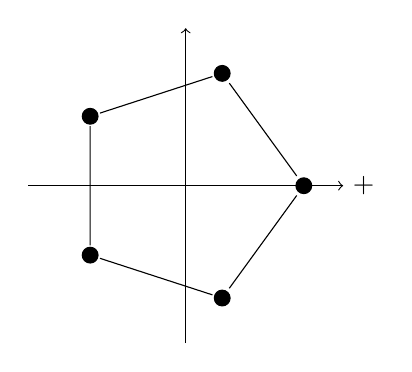
\begin{tikzpicture}
\draw[fill] (000:15mm) circle (1mm) node (A0){};
\draw[fill] (072:15mm) circle (1mm) node (A2){};
\draw[fill] (144:15mm) circle (1mm) node (A4){};
\draw[fill] (216:15mm) circle (1mm) node (A6){};
\draw[fill] (288:15mm) circle (1mm) node (A8){};
\draw (A0) -- (A2) -- (A4) -- (A6) -- (A8) -- (A0);
\draw [->] (-2,0) -- (2,0) node[right](){$+$};
\draw [->] (0,-2) -- (0,2);
\end{tikzpicture}
%--------------------------------------------------------------------------
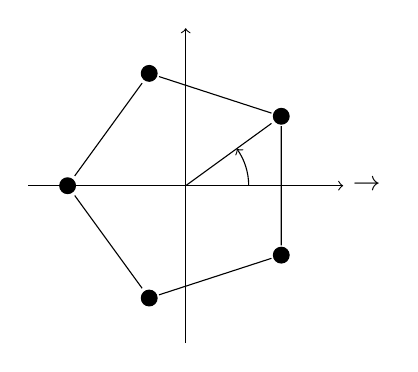
\begin{tikzpicture}
\draw[fill] (036:15mm) circle (1mm) node (A1){};
\draw[fill] (108:15mm) circle (1mm) node (A3){};
\draw[fill] (180:15mm) circle (1mm) node (A5){};
\draw[fill] (252:15mm) circle (1mm) node (A7){};
\draw[fill] (324:15mm) circle (1mm) node (A9){};
\draw (A1) -- (A3) -- (A5) -- (A7) -- (A9) -- (A1);
\draw(0,0) -- (A1);
\draw[->] (0.8,0) arc [start angle=0, radius=0.8cm,delta angle =36];
\draw [->] (-2,0) -- (2,0) node[right](){$\rightarrow$};
\draw [->] (0,-2) -- (0,2);
\end{tikzpicture}
%--------------------------------------------------------------------------
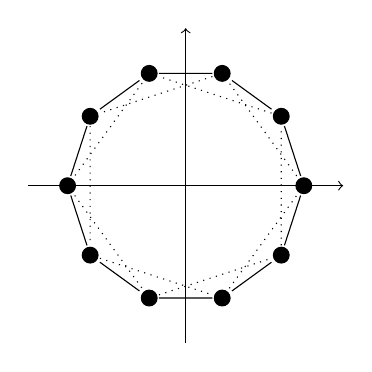
\begin{tikzpicture}
\draw[fill] (036:15mm) circle (1mm) node (A1){};
\draw[fill] (108:15mm) circle (1mm) node (A3){};
\draw[fill] (180:15mm) circle (1mm) node (A5){};
\draw[fill] (252:15mm) circle (1mm) node (A7){};
\draw[fill] (324:15mm) circle (1mm) node (A9){};
\draw[fill] (000:15mm) circle (1mm) node (A0){};
\draw[fill] (072:15mm) circle (1mm) node (A2){};
\draw[fill] (144:15mm) circle (1mm) node (A4){};
\draw[fill] (216:15mm) circle (1mm) node (A6){};
\draw[fill] (288:15mm) circle (1mm) node (A8){};
\draw[dotted] (A0) -- (A2) -- (A4) -- (A6) -- (A8) -- (A0);
\draw[dotted] (A1) -- (A3) -- (A5) -- (A7) -- (A9) -- (A1);
\draw (A0) -- (A1) -- (A2) -- (A3) -- (A4) -- (A5) -- (A6) -- (A7) -- (A8) -- (A9) -- (A0);
\draw [->] (-2,0) -- (2,0);
\draw [->] (0,-2) -- (0,2);
\end{tikzpicture}\]
%--------------------------------------------------------------------------

%--------------------------------------------------------------------------
\begin{align*}
c_k&=\frac 1N\sum_{p=0}^{N-1} e^{-2ipk\pi/N}x_p
=\frac 1{2M}\sum_{p=0}^{2M-1} e^{-2ipk\pi/2M}x_p\hbox{ en posant N=2M}
\\ &
=\frac 1{2M}\sum_{p=0,\ p \hbox{ pair}}^{2M-1} e^{-2ipk\pi/2M}x_p + \frac 1{2M}\sum_{p=0,\ p \hbox{ impair}}^{2M-1} e^{-2ipk\pi/2M}x_p
\\ &
=\frac 1{2M}\sum_{q=0}^{M-1} e^{-2i(2q)k\pi/2M}x_{2q} + \frac 1{2M}\sum_{q=0}^{M-1} e^{-2i(2q+1)k\pi/2M}x_{2q+1}
\\ &
=\frac 1{2M}\sum_{q=0}^{M-1} e^{-2iqk\pi/M}x_{2q} + \frac {e^{-2ik\pi/2M}}{2M}\sum_{q=0}^{M-1} e^{-2iqk\pi/M}x_{2q+1}
\end{align*}
%--------------------------------------------------------------------------

Si on note $X'$ la suite $(x_0,x_2,\ldots,x_{2N-2})$ et $X''$ la suite $(x_1,x_3,\ldots,x_{2N-1})$, les coefficients de la transformée de Fourier de $X'$ et $X''$, de longueur $M$, sont, pour $0\le k < M$,
%--------------------------------------------------------------------------
\begin{align*}
c'_k&=\frac 1{M}\sum_{q=0}^{M-1} e^{-2iqk\pi/M}x'_{q}=\frac 1{M}\sum_{q=0}^{M-1} e^{-2iqk\pi/M}x_{2q}\\
c''_k&=\frac 1{M}\sum_{q=0}^{M-1} e^{-2iqk\pi/M}x''_{q}=\frac 1{M}\sum_{q=0}^{M-1} e^{-2iqk\pi/M}x_{2q+1}
\end{align*}
%--------------------------------------------------------------------------

On a donc $c_k = \frac 12\bigl(c'_k + e^{-2ik\pi/2M} c''_k\bigr)$ pour $0\le k < M$.

\medskip

Pour $k$ compris entre $M$ et $N-1$ on pose $k = k' + M$.

On trouve alors, en utilisant $e^{-2iqM\pi/M}=1$ et $e^{-2iM\pi/2M}=-1$,
%--------------------------------------------------------------------------
\begin{align*}
c_k
&
=\frac 1{2M}\sum_{q=0}^{M-1} e^{-2iq(k'+M)\pi/M}x'_q + \frac {e^{-2i(k'+M)\pi/2M}}{2M}\sum_{q=0}^{M-1} e^{-2iq(k'+M)\pi/M}x''_q
\\&
=\frac 1{2M}\sum_{q=0}^{M-1} e^{-2iqk'\pi/M}x'_q + \frac {-e^{-2ik'\pi/2M}}{2M}\sum_{q=0}^{M-1} e^{-2iql\pi/M}x''_q
=\frac 12\bigl(c'_l - e^{-2il\pi/N} c''_l\bigr)
\end{align*}
%--------------------------------------------------------------------------
%--------------------------------------------------------------------------
\subsection{Algorithme}
%--------------------------------------------------------------------------
%--------------------------------------------------------------------------
Pour pouvoir effectuer la division par 2 à chaque étape nous allons supposer que 
\begin{center}
{\bf N est une puissance de 2}.
\end{center}

On arrive ainsi à un calcul récursif.

Pour calculer les coefficients à partir d'une suite de longueur $N$,

\begin{enumerate}
  \item Si $N=1$ on a $c_0=x_0$
  \item Sinon on décompose la suite en deux suite de taille $M=N/2$,

$X'=(x_0,x_2,\ldots,x_{2N-2})$ et $X''=(x_1,x_3,\ldots,x_{2N-1})$
\item On calcule les coefficients des suites $X'$ et $X''$
\item On calcule $c_k = \frac 12\bigl(c'_k + e^{-2ik\pi/N} c''_k\bigr)$ et $c_{k+M}=\frac 12\bigl(c'_k - e^{-2ik\pi/N} c''_k\bigr)$ pour $0\le k < M$.
\end{enumerate}

\subsubsection{Complexité}
On note $C(N)$ le nombre de multiplications nécessaires pour calculer la suite des $c_k$.

On a $C(N) = 2 C(M)+ 4 M$ et $C(1) = 0$.

Si on pose $N=2^p$ (d'où $M = 2^{p-1}$) on a $C(2^p) = 2C(2^{p-1})+4.2^{p-1}$.

On pose $C(2^p) = 2^p u_p$, on a $u_p=u_{p-1}+2$ et $u_0=0$ d'où $u_p=2p$ puis

$C(2^p)=2p2^p = 2\log_2(N)N$ qui est infiniment plus petit que le $N^2$ de la méthode ci-dessus.

\medskip

On calcule ici le produit d'une matrice par un vecteur avec une complexité quasi-linéaire !
%--------------------------------------------------------------------------
\begin{Exercise}\it Montrer que le nombre d'additions est $\log_2(N)N$, le nombre de calculs d'une exponentielle complexe est $\frac 12\log_2(N)N$ et le nombre d'affectations est $2\log_2(N)N$.
\end{Exercise}
%--------------------------------------------------------------------------
\begin{Answer} 
On a $C_{add}(2M) = 2C_{add}(M)+2M$, $C_{exp}(2M) = 2C_{exp}(M)+M$, $C_{aff}(2M) = 2C_{aff}(M)+2M$ d'où les résultats avec la même méthode que ci-dessus.

On remarquera que, dans le cas de l'algorithme simple, on a $C_{add}(N)) = N^2$, $C_{exp}(N)) = N^2$ et $C_{aff}(N)) = N$, seule la complexité en nombre d'affectation a (légèrement) augmenté.
\end{Answer}
%--------------------------------------------------------------------------
%--------------------------------------------------------------------------
\subsection{Transformation inverse}\label{iTFR} 
%--------------------------------------------------------------------------
%--------------------------------------------------------------------------
La transformation de Fourier inverse consiste à déterminer les $x_p$ à partir des $c_k$ ; cela correspond aux formules initiales.

On connaît la suite des $c_k$ avec $0 \le k < N=2M$.

On veut calculer $\displaystyle x_p=\sum_{k=0}^{N-1}c_ke^{2ip\pi k/N}$ pour $0\le p < N$.

On définit $d_k=c_{2k}$ et $d'_k=c_{2k+1}$ pour $0\le k< M$.

On suppose qu'on a calculé $\displaystyle y_p=\sum_{k=0}^{M-1}d_ke^{2ip\pi k/M}$ et $\displaystyle y'_p=\sum_{k=0}^{N-1}d'_ke^{2ip\pi k/M}$ pour $0\le p < M$.
%--------------------------------------------------------------------------
\begin{Exercise}\it 
Prouver qu'on a $x_p = y_p+e^{2ik\pi/N}y'_p$ et $x_{p+M} = y_p-e^{2ik\pi/N}y'_p$ pour $0\le p < M$.
\end{Exercise}
%--------------------------------------------------------------------------
\begin{Answer}
\begin{align*}
x_p
&
=\sum_{k=0}^{N-1} e^{2ipk\pi/N}c_k
=\sum_{k=0}^{2M-1} e^{2ipk\pi/2M}c_k
\\ &
=\sum_{l=0}^{M-1} e^{2ip(2l)\pi/2M}c_{2l} + \sum_{q=0}^{M-1} e^{2ip(2l+1)\pi/2M}c_{2l+1}
\\ &
=\sum_{l=0}^{M-1} e^{2ipl\pi/M}d_l + e^{2ip\pi/N}\sum_{l=0}^{M-1} e^{2ipl\pi/M}d'_l
\end{align*}
\newpage
\end{Answer}
%--------------------------------------------------------------------------
%--------------------------------------------------------------------------
%--------------------------------------------------------------------------
\section{Programmation}
%--------------------------------------------------------------------------
%--------------------------------------------------------------------------
%--------------------------------------------------------------------------
\begin{itemize}
  \item Pour accélérer les calculs on utilisera des tableaux {\tt numpy} : ils sont créés en convertissant une liste ({\tt np.array(liste)}) ou en affectant les valeurs d'une liste définie par {\tt np.zeros(taille)}.

\item On rappelle qu'on peut additionner ou multiplier deux tableaux de même longueur et multiplier un tableau par une constante sans avoir besoin d'écrire une boucle {\tt for}.

\item Ces tableaux, comme les listes usuelles, permettent l'extraction sous la forme {\tt liste[a:b:c]} qui extrait les termes {\tt liste[a+kc]} avec $k\ge 0$ et $a+kc <b$.

\item Les nombres complexes sont utilisables nativement dans python. Le nombre complexe de module 1 et d'argument $\frac \pi2$ est noté {\tt 1j}.

\item On peut définir un nombre complexe sous la forme {\tt 0.6+0.8j} si ses parties réelles et imaginaires sont explicites mais si les composantes sont des variables il faut employer {\tt a +b*1j} ou {\tt complex(a,b)} qui renvoie $a+ib$.

\item Les fonctions {\tt numpy} acceptent des variables complexes. En particulier on peut définir le nombre complexe $e^{i\theta}$ par \type{np.exp(theta*1j)}

\item Si on veut un tableau qui peut contenir des complexes on l'initialise en donnant son type :
\begin{lstlisting}
np.zeros(taille, dtype=complex)
\end{lstlisting}
\end{itemize}
%--------------------------------------------------------------------------
%--------------------------------------------------------------------------
\subsection{Implémentation de l'algorithme}
%--------------------------------------------------------------------------
%--------------------------------------------------------------------------
\begin{Exercise}\it Écrire une fonction {\tt separer(liste)} qui reçoit une liste de taille $N=2M$ et qui renvoie les deux listes de taille $M$ formées des éléments d'indices respectivement pairs et impairs de la liste initiale dans le même ordre.
\end{Exercise}
%--------------------------------------------------------------------------
\begin{Answer}
\begin{lstlisting}
def separer(liste):
    lPairs = liste[::2]
    lImpairs = liste[1::2]
    return lPairs, lImpairs
\end{lstlisting}
\end{Answer}
%--------------------------------------------------------------------------
\begin{Exercise}\it 
Écrire une fonction {\tt listeExp(N)} qui reçoit un entier pair $N$ et qui renvoie le tableau {\tt numpy} de taille $N/2$ dont chaque composante d'indice $k$ est $e^{-2ik\pi/N}$.
\end{Exercise}
%--------------------------------------------------------------------------
\begin{Answer}
\begin{lstlisting}
def listeExp(N):
    M = N//2
    expo = np.zeros(M,dtype=complex)
    for k in range(M):
        theta = -k*np.pi/M
        expo[k] = np.exp(theta*1j)
    return expo
\end{lstlisting}
On peut, ici aussi, éviter les boucles.
\begin{lstlisting}
def listeExp(N):
    M = N//2
    A = np.linspace(0,M-1,M)
    Theta = -A*np.pi/M
    return np.exp(Theta*1j)
\end{lstlisting}
\end{Answer}
%--------------------------------------------------------------------------
\begin{Exercise}\it Écrire une fonction {\tt TFR(liste)} qui reçoit une liste de taille $2^p$ et qui renvoie la liste (complexe) de ses coefficients de Fourier en utilisant l'algorithme rapide vu ci-dessus.

On ne vérifiera pas que la taille est une puissance de 2.
\end{Exercise}
%--------------------------------------------------------------------------
\begin{Answer}
\begin{lstlisting}
def TFR(liste):
    N = len(liste)
    if N == 1:
        return np.array([liste[0]+0j])
    else:
        M = N//2
        C= np.zeros(N,dtype=complex)
        X1, X2 = separer(liste)
        C1 = TFR(X1)
        C2 = TFR(X2)
        E = listeExp(N)
        C[:M] = (C1 + E*C2)/2
        C[M:] = (C1 - E*C2)/2
        return C
\end{lstlisting}
\end{Answer}
%--------------------------------------------------------------------------
%--------------------------------------------------------------------------
\subsection{Quelques spectres}
%--------------------------------------------------------------------------
%--------------------------------------------------------------------------
Dans cette partie nous allons construire quelques signaux et les analyser.

Pour que les calculs soient rapides les échantillons seront de taille $N = 1024 = 2^{10}$.

Si on veut une valeur réelle des fréquences calculées il faut connaître la durée de l'échantillon donc la fréquence d'échantillonnage : on choisit $f_e = 1000\ Hz$. La durée totale est donc $\frac N{f_e}=1,024\ s$, le pas de temps est $dt = \frac 1{f_e}=1\ ms$, le pas des fréquences, $df$, est l'inverse de la durée.

\begin{lstlisting}
N = 1024     # nombre de pas
fe = 1000    # fréquence d'échantillonnage
duree = N/fe # durée de l'échantillonnage
dt = 1/fe    # temps entre deux mesures
df = 1/duree # fréquence de base
\end{lstlisting}

\newpage

Pour tracer les représentations on pourra utiliser des tableaux {\tt numpy} pour les abscisses : {\tt temps} pour les signaux et {\tt freq} pour les composantes de la transformée.

On affichera, les fréquences supérieures à la fréquence limite sous la forme de fréquences négatives.
\begin{lstlisting}
U = np.arange(N)    # tableau de taille N, de 0 à N-1
temps = U*dt
freq = (U-N//2)*df
\end{lstlisting}

On définit une fonction pour le signal, par exemple

\begin{lstlisting}
f = 25
def fonction(t):
    return np.sin(2*np.pi*f*t)
\end{lstlisting}

Certaines fonctions ne sont pas directement applicables à un tableau {\tt numpy}, par exemple celles qui effectuent un test ({\tt if}). On peut les transformer pour qu'elles le deviennent avec l'instruction {\tt fonction = np.vectorize(fonction1)}.

Voici un modèle simple pour dessiner le signal et sa transformée.

On notera que l'on calcule les modules des coefficients pour l'affichage.

\begin{lstlisting}
signal = fonction(temps)
coef = TFR(signal)
coefR = np.zeros(N)
coefR[:N//2] = abs(coef)[N//2:]
coefR[N//2:] = abs(coef)[:N//2]

plt.clf()  # On efface

plt.subplot(2,1,1)       # Premier dessin, le signal
plt.plot(temps,signal)   # Tracé
plt.xlim((0,1.05))       # On ajuste l'axe horizontal
plt.xlabel("Temps [s]")  # Label pour les abscisses
plt.ylabel("Signal")     # Label pour les ordonnées

plt.subplot(2,1,2)       # Second dessin, la transformée
plt.plot(freq,coefR)
plt.xlabel("Fréquence [Hz]")
plt.ylabel("Coefficients")

plt.show()               # On fait dessiner
\end{lstlisting}

La dernière instruction n'est utile que si on n'est pas en mode interactif. On se place en mode interactif avec la commande {\tt plt.ion()}, on en sort avec la commande {\tt plt.ioff()}.
%--------------------------------------------------------------------------
\begin{Exercise}\it Déterminer un signal et sa transformée dans les cas suivants.
\begin{enumerate}
  \item $\sin(2\pi f t)$, on pourra choisir $f=62,5$ puis $f=50$.

  Donner une explication à la différence des spectres.
  \item $\sin(2\pi f_1 t) + \sin(2\pi f_2 t)$ puis $\sin(2\pi f_1 t).\sin(2\pi f_2 t)$.
  \item $|\sin(2\pi f t)|$.
  \item Un signal en dents-de-scie\footnote{{\tt x\%y} donne la partie fractionnaire de $\frac xy$ quand $x$ ou $y$ est un réel.}.
  \item Un signal triangulaire.
  \item Un signal carré.
  \end{enumerate}
\end{Exercise}
%--------------------------------------------------------------------------
\begin{Answer}
\begin{enumerate}
  \item Pour $f=62,5$ la longueur est un multiple entier de la fréquence : il n'y a qu'une paire de coefficients non nuls. Dans le cas général il apparaît des coefficients non négligeables autour de la fréquence.
  \item La linéarisation du produit fait apparaître des signaux de fréquence $f_1+f_2$ et $f_1-f_2$
  \item On notera que $c_0$ est non nul, le signal a une composante constante.
\item
\begin{lstlisting}
f = 10
def fn(t):
    T = 1/f
    u = t%T
    return 2*f*u-1 # de -1 à 1

fonction = np.vectorize(fn)
\end{lstlisting}

\item
\begin{lstlisting}
f = 100
def fn(t):
    T = 1/f
    u = t%T
    return abs(2*f*u-1)

fonction = np.vectorize(fn)
\end{lstlisting}

On remarque que seuls les multiples impairs de la fréquence apparaissent.
\begin{lstlisting}
f = 10
def fn(t):
    T = 1/f
    u = t%T
    if u < T/2:
        return 1
    else:
        return -1

fonction = np.vectorize(fn)
\end{lstlisting}

On peut aussi utiliser {\tt np.sign(np.sin(2*np.pi*f*t))}

  \end{enumerate}
\end{Answer}
%--------------------------------------------------------------------------
\newpage
%--------------------------------------------------------------------------
\subsection{Transformation inverse}
%--------------------------------------------------------------------------
%--------------------------------------------------------------------------
La transformation inverse a été vue à la partie \ref{iTFR}. 

Elle se calcule de la même façon que la transformation directe à l'exception de 2 changements.
\begin{itemize}
 \item On ne divise plus par 2 les reconstitutions des coefficients.
 \item On multiplie par une exponentielle de la forme $e^{2ik\pi/N}$ au lieu de $e^{-2ik\pi/N}$ 
\end{itemize}
%--------------------------------------------------------------------------
\begin{Exercise}\it Écrire une fonction {\tt listeExpInv(N)} qui reçoit un entier pair $N$ et qui renvoie le tableau 
{\tt numpy} de taille $N/2$ dont chaque composante d'indice $k$ est $e^{2ik\pi/N}$.
\end{Exercise}
%--------------------------------------------------------------------------
\begin{Answer}
\begin{lstlisting}
def listeExpInv(N):
    M = N//2
    A = np.linspace(0,M-1,M)
    Theta = A*np.pi/M
    return np.exp(Theta*1j)
\end{lstlisting}
\end{Answer}
%--------------------------------------------------------------------------
\begin{Exercise}\it 
Écrire une fonction {\tt invTFR(liste)} qui reçoit une liste de taille $2^p$ représentant les 
coefficients de Fourier et qui renvoie la liste des valeurs en utilisant l'algorithme rapide vu ci-dessus.
\end{Exercise}
%--------------------------------------------------------------------------
\begin{Answer}
\begin{lstlisting}
def invTFR(liste):
    N = len(liste)
    if N == 1:
        return np.array([liste[0]+0j])
    else:
        M = N//2
        X= np.zeros(N,dtype=complex)
        C1, C2 = separer(liste)
        X1 = invTFR(C1)
        X2 = invTFR(C2)
        E = listeExp2(N)
        X[:M] = X1 + E*X2
        X[M:] = X1 - E*X2
        return X
\end{lstlisting}
\newpage
\end{Answer}
%--------------------------------------------------------------------------
%--------------------------------------------------------------------------
\subsection{Filtrage}
%--------------------------------------------------------------------------
%--------------------------------------------------------------------------
Une application de la transformation de Fourier est le filtrage :
\begin{itemize}
 \item on transforme un signal,
 \item on modifie les coefficients selon la fréquence,
 \item on calcule la transformée inverse.
\end{itemize}

On propose deux sortes de filtrages passe-bas :
\begin{enumerate}
 \item on enleve les fréquences hautes, par exemple entre {\tt N//6} et {\tt N-N//6},
 \item on atténue les fréquences hautes, par exemple en multipliant par une liste qui décroit de 1 à 0 entre 0 et {\tt N//2} 
 puis croît de 0 à 1 entre {\tt N//2} et {\tt N}.
\end{enumerate}
%--------------------------------------------------------------------------
\begin{Exercise}\it Expérimenter ces deux types de filtres avec des signaux carrés, triangulaires ou en dents-de-scie.
\end{Exercise}
%--------------------------------------------------------------------------
\begin{Answer}
\begin{lstlisting}
N = 1024    # nombre de pas
fe = 1000    # frequence d'échantillonnage
duree = N/fe # durée de l'échantillonnage
dt = 1/fe    # temps entre deux mesures
df = 1/duree # fréquence de base
  
U = np.arange(N)    # tableau de taille N, de 0 à N-1
temps = U*dt
freq = (U-N//2)*df

f = 10
# Carré
# def fn(t):
#     T = 1/f
#     u = t%T
#     if u < T/2:
#         return 1
#     else:
#        return -1

# Dents de scie
def fn(t):
    T = 1/f
    u = t%T
    return 2*f*u-1 # de -1 à 1

# Triangle
# def fn(t):
#     T = 1/f
#     u = t%T
#     return abs(2*f*u-1)

fonction = np.vectorize(fn)

signal = fonction(temps)
coef = TFR(signal)

# Filtrage doux
# coef = coef*(abs(2*U-N)/N)**4

# Filtrage raide
d = N//6
coef[d:N-d]=0 

signal1 = invTFR(coef).real
signal2 = invTFR(coef).imag
\end{lstlisting}
\end{Answer}
% %--------------------------------------------------------------------------
% %--------------------------------------------------------------------------
% \subsection{Question supplémentaire}
% %--------------------------------------------------------------------------
% %--------------------------------------------------------------------------
% Le module {\tt scipy} contient un sous-module qui permet de lire et écrire les fichiers sons enregistrés sous le format {\bf wav}.
%
% {\tt import scipy.io.wavfile as wav} importe les fonctions de ce module.
%
% \begin{itemize}
%  \item {\tt son = wav.read("chemin/vers/un/fichier/a\_lire.wav"} charge un fichier {\tt a\_lire.wav} sous la forme d'un couple
%  {\tt son = (fe,signal)} où {\tt fe} est la fréquence d'échantillonage et {\tt signal} est un tableau {\tt numpy} contenant les valeurs du signal aux
%  différents temps d'échantillonage.
%  \item {\tt wav.write("chemin/vers/un/fichier/a\_ecrire.wav",fe,signal)} sauvegarde le tableau {\tt numpy} associé à la variable
%  {\tt signal} sous la forme d'un fichier {\tt a\_ecrire.wav} enregistré à la fréquence d'échantillonnage {\tt fe}. 
%
% \end{itemize}
% %--------------------------------------------------------------------------
% \begin{Exercise}\it Il y a un fichier {\tt MLKing.wav} dans le dossier public. Celui-ci un extrait d'un discours celèbre
% pertubé par un signal périodique. Le but est de fournir un fichier {\bf wav} nettoyé.
% \end{Exercise}
% %--------------------------------------------------------------------------
% \begin{Answer}
% \begin{lstlisting}
%
% \end{lstlisting}
% \end{Answer}
%
\newpage
%--------------------------------------------------------------------------
%--------------------------------------------------------------------------
%--------------------------------------------------------------------------
